% Options for packages loaded elsewhere
\PassOptionsToPackage{unicode}{hyperref}
\PassOptionsToPackage{hyphens}{url}
\PassOptionsToPackage{dvipsnames,svgnames,x11names}{xcolor}
%
\documentclass[
  letterpaper,
  DIV=11,
  numbers=noendperiod]{scrreprt}

\usepackage{amsmath,amssymb}
\usepackage{iftex}
\ifPDFTeX
  \usepackage[T1]{fontenc}
  \usepackage[utf8]{inputenc}
  \usepackage{textcomp} % provide euro and other symbols
\else % if luatex or xetex
  \usepackage{unicode-math}
  \defaultfontfeatures{Scale=MatchLowercase}
  \defaultfontfeatures[\rmfamily]{Ligatures=TeX,Scale=1}
\fi
\usepackage{lmodern}
\ifPDFTeX\else  
    % xetex/luatex font selection
\fi
% Use upquote if available, for straight quotes in verbatim environments
\IfFileExists{upquote.sty}{\usepackage{upquote}}{}
\IfFileExists{microtype.sty}{% use microtype if available
  \usepackage[]{microtype}
  \UseMicrotypeSet[protrusion]{basicmath} % disable protrusion for tt fonts
}{}
\makeatletter
\@ifundefined{KOMAClassName}{% if non-KOMA class
  \IfFileExists{parskip.sty}{%
    \usepackage{parskip}
  }{% else
    \setlength{\parindent}{0pt}
    \setlength{\parskip}{6pt plus 2pt minus 1pt}}
}{% if KOMA class
  \KOMAoptions{parskip=half}}
\makeatother
\usepackage{xcolor}
\setlength{\emergencystretch}{3em} % prevent overfull lines
\setcounter{secnumdepth}{2}
% Make \paragraph and \subparagraph free-standing
\ifx\paragraph\undefined\else
  \let\oldparagraph\paragraph
  \renewcommand{\paragraph}[1]{\oldparagraph{#1}\mbox{}}
\fi
\ifx\subparagraph\undefined\else
  \let\oldsubparagraph\subparagraph
  \renewcommand{\subparagraph}[1]{\oldsubparagraph{#1}\mbox{}}
\fi

\usepackage{color}
\usepackage{fancyvrb}
\newcommand{\VerbBar}{|}
\newcommand{\VERB}{\Verb[commandchars=\\\{\}]}
\DefineVerbatimEnvironment{Highlighting}{Verbatim}{commandchars=\\\{\}}
% Add ',fontsize=\small' for more characters per line
\usepackage{framed}
\definecolor{shadecolor}{RGB}{241,243,245}
\newenvironment{Shaded}{\begin{snugshade}}{\end{snugshade}}
\newcommand{\AlertTok}[1]{\textcolor[rgb]{0.68,0.00,0.00}{#1}}
\newcommand{\AnnotationTok}[1]{\textcolor[rgb]{0.37,0.37,0.37}{#1}}
\newcommand{\AttributeTok}[1]{\textcolor[rgb]{0.40,0.45,0.13}{#1}}
\newcommand{\BaseNTok}[1]{\textcolor[rgb]{0.68,0.00,0.00}{#1}}
\newcommand{\BuiltInTok}[1]{\textcolor[rgb]{0.00,0.23,0.31}{#1}}
\newcommand{\CharTok}[1]{\textcolor[rgb]{0.13,0.47,0.30}{#1}}
\newcommand{\CommentTok}[1]{\textcolor[rgb]{0.37,0.37,0.37}{#1}}
\newcommand{\CommentVarTok}[1]{\textcolor[rgb]{0.37,0.37,0.37}{\textit{#1}}}
\newcommand{\ConstantTok}[1]{\textcolor[rgb]{0.56,0.35,0.01}{#1}}
\newcommand{\ControlFlowTok}[1]{\textcolor[rgb]{0.00,0.23,0.31}{#1}}
\newcommand{\DataTypeTok}[1]{\textcolor[rgb]{0.68,0.00,0.00}{#1}}
\newcommand{\DecValTok}[1]{\textcolor[rgb]{0.68,0.00,0.00}{#1}}
\newcommand{\DocumentationTok}[1]{\textcolor[rgb]{0.37,0.37,0.37}{\textit{#1}}}
\newcommand{\ErrorTok}[1]{\textcolor[rgb]{0.68,0.00,0.00}{#1}}
\newcommand{\ExtensionTok}[1]{\textcolor[rgb]{0.00,0.23,0.31}{#1}}
\newcommand{\FloatTok}[1]{\textcolor[rgb]{0.68,0.00,0.00}{#1}}
\newcommand{\FunctionTok}[1]{\textcolor[rgb]{0.28,0.35,0.67}{#1}}
\newcommand{\ImportTok}[1]{\textcolor[rgb]{0.00,0.46,0.62}{#1}}
\newcommand{\InformationTok}[1]{\textcolor[rgb]{0.37,0.37,0.37}{#1}}
\newcommand{\KeywordTok}[1]{\textcolor[rgb]{0.00,0.23,0.31}{#1}}
\newcommand{\NormalTok}[1]{\textcolor[rgb]{0.00,0.23,0.31}{#1}}
\newcommand{\OperatorTok}[1]{\textcolor[rgb]{0.37,0.37,0.37}{#1}}
\newcommand{\OtherTok}[1]{\textcolor[rgb]{0.00,0.23,0.31}{#1}}
\newcommand{\PreprocessorTok}[1]{\textcolor[rgb]{0.68,0.00,0.00}{#1}}
\newcommand{\RegionMarkerTok}[1]{\textcolor[rgb]{0.00,0.23,0.31}{#1}}
\newcommand{\SpecialCharTok}[1]{\textcolor[rgb]{0.37,0.37,0.37}{#1}}
\newcommand{\SpecialStringTok}[1]{\textcolor[rgb]{0.13,0.47,0.30}{#1}}
\newcommand{\StringTok}[1]{\textcolor[rgb]{0.13,0.47,0.30}{#1}}
\newcommand{\VariableTok}[1]{\textcolor[rgb]{0.07,0.07,0.07}{#1}}
\newcommand{\VerbatimStringTok}[1]{\textcolor[rgb]{0.13,0.47,0.30}{#1}}
\newcommand{\WarningTok}[1]{\textcolor[rgb]{0.37,0.37,0.37}{\textit{#1}}}

\providecommand{\tightlist}{%
  \setlength{\itemsep}{0pt}\setlength{\parskip}{0pt}}\usepackage{longtable,booktabs,array}
\usepackage{calc} % for calculating minipage widths
% Correct order of tables after \paragraph or \subparagraph
\usepackage{etoolbox}
\makeatletter
\patchcmd\longtable{\par}{\if@noskipsec\mbox{}\fi\par}{}{}
\makeatother
% Allow footnotes in longtable head/foot
\IfFileExists{footnotehyper.sty}{\usepackage{footnotehyper}}{\usepackage{footnote}}
\makesavenoteenv{longtable}
\usepackage{graphicx}
\makeatletter
\def\maxwidth{\ifdim\Gin@nat@width>\linewidth\linewidth\else\Gin@nat@width\fi}
\def\maxheight{\ifdim\Gin@nat@height>\textheight\textheight\else\Gin@nat@height\fi}
\makeatother
% Scale images if necessary, so that they will not overflow the page
% margins by default, and it is still possible to overwrite the defaults
% using explicit options in \includegraphics[width, height, ...]{}
\setkeys{Gin}{width=\maxwidth,height=\maxheight,keepaspectratio}
% Set default figure placement to htbp
\makeatletter
\def\fps@figure{htbp}
\makeatother

% Soul package to handle highlighting (see hl.py3 filter)
\usepackage{soul}

% For tables generated by the gt package
\usepackage{colortbl}
\KOMAoption{captions}{tableheading}
\makeatletter
\@ifpackageloaded{bookmark}{}{\usepackage{bookmark}}
\makeatother
\makeatletter
\@ifpackageloaded{caption}{}{\usepackage{caption}}
\AtBeginDocument{%
\ifdefined\contentsname
  \renewcommand*\contentsname{Índice}
\else
  \newcommand\contentsname{Índice}
\fi
\ifdefined\listfigurename
  \renewcommand*\listfigurename{Lista de Figuras}
\else
  \newcommand\listfigurename{Lista de Figuras}
\fi
\ifdefined\listtablename
  \renewcommand*\listtablename{Lista de Tabelas}
\else
  \newcommand\listtablename{Lista de Tabelas}
\fi
\ifdefined\figurename
  \renewcommand*\figurename{Figura}
\else
  \newcommand\figurename{Figura}
\fi
\ifdefined\tablename
  \renewcommand*\tablename{Tabela}
\else
  \newcommand\tablename{Tabela}
\fi
}
\@ifpackageloaded{float}{}{\usepackage{float}}
\floatstyle{ruled}
\@ifundefined{c@chapter}{\newfloat{codelisting}{h}{lop}}{\newfloat{codelisting}{h}{lop}[chapter]}
\floatname{codelisting}{Listagem}
\newcommand*\listoflistings{\listof{codelisting}{Lista de Listagens}}
\makeatother
\makeatletter
\makeatother
\makeatletter
\@ifpackageloaded{caption}{}{\usepackage{caption}}
\@ifpackageloaded{subcaption}{}{\usepackage{subcaption}}
\makeatother
\ifLuaTeX
\usepackage[bidi=basic]{babel}
\else
\usepackage[bidi=default]{babel}
\fi
\babelprovide[main,import]{portuguese}
% get rid of language-specific shorthands (see #6817):
\let\LanguageShortHands\languageshorthands
\def\languageshorthands#1{}
\ifLuaTeX
  \usepackage{selnolig}  % disable illegal ligatures
\fi
\usepackage{bookmark}

\IfFileExists{xurl.sty}{\usepackage{xurl}}{} % add URL line breaks if available
\urlstyle{same} % disable monospaced font for URLs
\hypersetup{
  pdftitle={Comparando listas e rankings},
  pdfauthor={Fernando Náufel},
  pdflang={pt},
  colorlinks=true,
  linkcolor={blue},
  filecolor={Maroon},
  citecolor={Blue},
  urlcolor={Blue},
  pdfcreator={LaTeX via pandoc}}

\title{Comparando listas e rankings}
\author{Fernando Náufel}
\date{12/02/2024 16:27}

\begin{document}
\maketitle

% Bold title in callout boxes
% But we must be careful: if there are no callout boxes in the document,
% then package tcolorbox has NOT been loaded, and we must refrain from
% setting this up; hence the ifpackageloaded
\makeatletter
\@ifpackageloaded{tcolorbox}
{\tcbset{fonttitle=\bfseries}}
{}
\makeatother


\renewcommand*\contentsname{Índice}
{
\hypersetup{linkcolor=}
\setcounter{tocdepth}{2}
\tableofcontents
}
\bookmarksetup{startatroot}

\chapter*{Apresentação}\label{apresentauxe7uxe3o}
\addcontentsline{toc}{chapter}{Apresentação}

\markboth{Apresentação}{Apresentação}

???

\bookmarksetup{startatroot}

\chapter{\texorpdfstring{Listas e
\emph{rankings}}{Listas e rankings}}\label{listas-e-rankings}

\section{Problema}\label{problema}

Vamos trabalhar com listas e \emph{rankings} sujeitos às seguintes
condições:

\begin{itemize}
\item
  A {\hl{lista}} tem $k$ elementos, $k > 0$, {\hl{não ordenados}}.
\item
  O {\hl{\emph{ranking}}} tem $p$ elementos, $p \geq k$,
  {\hl{ordenados}}, {\hl{sem empates}}.
\item
  Todos os elementos da lista também pertencem ao \emph{ranking}.
\item
  O último elemento do \emph{ranking} sempre pertence à lista.
\item
  As identidades dos elementos do \emph{ranking} não importam --- i.e.,
  eles são indistinguíveis, a não ser por pertencerem ou não à lista (e
  pela ordem que ocupam no \emph{ranking}, claro).
\end{itemize}

\section{\texorpdfstring{Criando
\emph{rankings}}{Criando rankings}}\label{criando-rankings}

\subsection{Representação}\label{sec-repr}

Considere naturais $k > 0$ e $p \geq k$.

{\hl{Podemos representar um \emph{ranking} através de um \emph{string}
contendo $k$ caracteres ``{\mbox{\texttt{x}}}'' e $p - k$ caracteres
``{\mbox{\texttt{-}}}''}}.

``\texttt{x}'' representa uma posição ocupada por um elemento da lista.

``\texttt{-}'' representa uma posição ocupada por um elemento que não
está na lista.

Você pode usar a função \texttt{rk()} para criar um \emph{ranking},
passando um \emph{string} da forma acima:

\begin{Shaded}
\begin{Highlighting}[]
\FunctionTok{rk}\NormalTok{(}\StringTok{\textquotesingle{}xx{-}{-}x\textquotesingle{}}\NormalTok{)}
\end{Highlighting}
\end{Shaded}

\begin{verbatim}
ranking: [✔✔••✔] (p = 5, k = 3)
\end{verbatim}

R vai mostrar o \emph{ranking} com os valores de $k$ e $p$ e com
caracteres unicode (por default). Se quiser ver o \emph{ranking} com
caracteres ASCII, use a função \texttt{print} com o argumento
\texttt{unicode\ =\ FALSE}:

\begin{Shaded}
\begin{Highlighting}[]
\FunctionTok{print}\NormalTok{(}\FunctionTok{rk}\NormalTok{(}\StringTok{\textquotesingle{}xx{-}{-}x\textquotesingle{}}\NormalTok{), }\AttributeTok{unicode =} \ConstantTok{FALSE}\NormalTok{)}
\end{Highlighting}
\end{Shaded}

\begin{verbatim}
ranking: [xx--x] (p = 5, k = 3)
\end{verbatim}

\subsection{\texorpdfstring{Quantidade de
\emph{rankings}}{Quantidade de rankings}}\label{quantidade-de-rankings}

Dados $k > 0$ e $p \geq k$ fixos, quantos \emph{rankings} existem?

Para montar um \emph{ranking}:

\begin{enumerate}
\def\labelenumi{\arabic{enumi}.}
\item
  Sabemos que a última posição é ocupada por alguém da lista.
\item
  Só resta escolher as posições dos $k - 1$ elementos restantes da lista
  dentre as $p - 1$ posições restantes no \emph{ranking}, o que dá
  $\binom{p - 1}{k - 1}$ escolhas.
\end{enumerate}

Assim, a quantidade total de \emph{rankings} para $k$ e $p$ dados é

\[
\binom{p - 1}{k - 1}
\]

Por exemplo, para $k = 3, p = 5$, os $\binom{4}{2} = 6$ \emph{rankings}
possíveis são

\begin{itemize}
\tightlist
\item
  \texttt{xx-\/-x}
\item
  \texttt{x-x-x}
\item
  \texttt{x-\/-xx}
\item
  \texttt{-xx-x}
\item
  \texttt{-x-xx}
\item
  \texttt{-\/-xxx}
\end{itemize}

A tabela a seguir (na verdade, um pedaço do triângulo de Pascal) mostra
as quantidades de \emph{rankings} possíveis para alguns valores de $k$ e
$p$:

\begin{longtable*}{l|rrrrrrrrrr}
\toprule
\multicolumn{1}{l}{} & \multicolumn{10}{c}{\(k\)} \\ 
\cmidrule(lr){2-11}
\multicolumn{1}{l}{\(p\)} & 1 & 2 & 3 & 4 & 5 & 6 & 7 & 8 & 9 & 10 \\ 
\midrule\addlinespace[2.5pt]
$1$ & $1$ &  &  &  &  &  &  &  &  &  \\ 
$2$ & $1$ & $1$ &  &  &  &  &  &  &  &  \\ 
$3$ & $1$ & $2$ & $1$ &  &  &  &  &  &  &  \\ 
$4$ & $1$ & $3$ & $3$ & $1$ &  &  &  &  &  &  \\ 
$5$ & $1$ & $4$ & $6$ & $4$ & $1$ &  &  &  &  &  \\ 
$6$ & $1$ & $5$ & $10$ & $10$ & $5$ & $1$ &  &  &  &  \\ 
$7$ & $1$ & $6$ & $15$ & $20$ & $15$ & $6$ & $1$ &  &  &  \\ 
$8$ & $1$ & $7$ & $21$ & $35$ & $35$ & $21$ & $7$ & $1$ &  &  \\ 
$9$ & $1$ & $8$ & $28$ & $56$ & $70$ & $56$ & $28$ & $8$ & $1$ &  \\ 
$10$ & $1$ & $9$ & $36$ & $84$ & $126$ & $126$ & $84$ & $36$ & $9$ & $1$ \\ 
$11$ & $1$ & $10$ & $45$ & $120$ & $210$ & $252$ & $210$ & $120$ & $45$ & $10$ \\ 
$12$ & $1$ & $11$ & $55$ & $165$ & $330$ & $462$ & $462$ & $330$ & $165$ & $55$ \\ 
$13$ & $1$ & $12$ & $66$ & $220$ & $495$ & $792$ & $924$ & $792$ & $495$ & $220$ \\ 
$14$ & $1$ & $13$ & $78$ & $286$ & $715$ & $1.287$ & $1.716$ & $1.716$ & $1.287$ & $715$ \\ 
$15$ & $1$ & $14$ & $91$ & $364$ & $1.001$ & $2.002$ & $3.003$ & $3.432$ & $3.003$ & $2.002$ \\ 
$16$ & $1$ & $15$ & $105$ & $455$ & $1.365$ & $3.003$ & $5.005$ & $6.435$ & $6.435$ & $5.005$ \\ 
$17$ & $1$ & $16$ & $120$ & $560$ & $1.820$ & $4.368$ & $8.008$ & $11.440$ & $12.870$ & $11.440$ \\ 
$18$ & $1$ & $17$ & $136$ & $680$ & $2.380$ & $6.188$ & $12.376$ & $19.448$ & $24.310$ & $24.310$ \\ 
$19$ & $1$ & $18$ & $153$ & $816$ & $3.060$ & $8.568$ & $18.564$ & $31.824$ & $43.758$ & $48.620$ \\ 
$20$ & $1$ & $19$ & $171$ & $969$ & $3.876$ & $11.628$ & $27.132$ & $50.388$ & $75.582$ & $92.378$ \\ 
$21$ & $1$ & $20$ & $190$ & $1.140$ & $4.845$ & $15.504$ & $38.760$ & $77.520$ & $125.970$ & $167.960$ \\ 
$22$ & $1$ & $21$ & $210$ & $1.330$ & $5.985$ & $20.349$ & $54.264$ & $116.280$ & $203.490$ & $293.930$ \\ 
$23$ & $1$ & $22$ & $231$ & $1.540$ & $7.315$ & $26.334$ & $74.613$ & $170.544$ & $319.770$ & $497.420$ \\ 
$24$ & $1$ & $23$ & $253$ & $1.771$ & $8.855$ & $33.649$ & $100.947$ & $245.157$ & $490.314$ & $817.190$ \\ 
$25$ & $1$ & $24$ & $276$ & $2.024$ & $10.626$ & $42.504$ & $134.596$ & $346.104$ & $735.471$ & $1.307.504$ \\ 
$26$ & $1$ & $25$ & $300$ & $2.300$ & $12.650$ & $53.130$ & $177.100$ & $480.700$ & $1.081.575$ & $2.042.975$ \\ 
$27$ & $1$ & $26$ & $325$ & $2.600$ & $14.950$ & $65.780$ & $230.230$ & $657.800$ & $1.562.275$ & $3.124.550$ \\ 
$28$ & $1$ & $27$ & $351$ & $2.925$ & $17.550$ & $80.730$ & $296.010$ & $888.030$ & $2.220.075$ & $4.686.825$ \\ 
$29$ & $1$ & $28$ & $378$ & $3.276$ & $20.475$ & $98.280$ & $376.740$ & $1.184.040$ & $3.108.105$ & $6.906.900$ \\ 
$30$ & $1$ & $29$ & $406$ & $3.654$ & $23.751$ & $118.755$ & $475.020$ & $1.560.780$ & $4.292.145$ & $10.015.005$ \\ 
\bottomrule
\end{longtable*}

\subsection{\texorpdfstring{Criando um \emph{ranking} a partir de um
vetor}{Criando um ranking a partir de um vetor}}\label{criando-um-ranking-a-partir-de-um-vetor}

Em vez de especificar as $p$ posições do \emph{ranking}, {\hl{pode ser
mais compacto especificar as $k$ posições do \emph{ranking} que são
ocupadas por elementos da lista}}.

A função \texttt{rk()} também faz isso, recebendo um vetor numérico com
$k$ elementos.

\begin{Shaded}
\begin{Highlighting}[]
\FunctionTok{rk}\NormalTok{(}\FunctionTok{c}\NormalTok{(}\DecValTok{1}\NormalTok{, }\DecValTok{3}\NormalTok{, }\DecValTok{5}\NormalTok{, }\DecValTok{7}\NormalTok{))}
\end{Highlighting}
\end{Shaded}

\begin{verbatim}
ranking: [✔•✔•✔•✔] (p = 7, k = 4)
\end{verbatim}

Observe que as posições não precisam ser passadas em ordem:

\begin{Shaded}
\begin{Highlighting}[]
\FunctionTok{rk}\NormalTok{(}\FunctionTok{c}\NormalTok{(}\DecValTok{3}\NormalTok{, }\DecValTok{7}\NormalTok{, }\DecValTok{5}\NormalTok{, }\DecValTok{1}\NormalTok{))}
\end{Highlighting}
\end{Shaded}

\begin{verbatim}
ranking: [✔•✔•✔•✔] (p = 7, k = 4)
\end{verbatim}

A função detecta vetores que não podem representar \emph{rankings}:

\begin{Shaded}
\begin{Highlighting}[]
\FunctionTok{rk}\NormalTok{(}\FunctionTok{c}\NormalTok{(}\DecValTok{3}\NormalTok{, }\DecValTok{7}\NormalTok{, }\DecValTok{3}\NormalTok{, }\DecValTok{1}\NormalTok{))}
\end{Highlighting}
\end{Shaded}

\begin{verbatim}
Error in validate_rk(x): 
Valores precisam ser inteiros positivos, sem repetições.
\end{verbatim}

\begin{Shaded}
\begin{Highlighting}[]
\FunctionTok{rk}\NormalTok{(}\FunctionTok{c}\NormalTok{(}\DecValTok{5}\NormalTok{, }\DecValTok{7}\NormalTok{, }\DecValTok{3}\NormalTok{, }\FloatTok{1.5}\NormalTok{))}
\end{Highlighting}
\end{Shaded}

\begin{verbatim}
Error in validate_rk(x): 
Valores precisam ser inteiros positivos, sem repetições.
\end{verbatim}

\begin{Shaded}
\begin{Highlighting}[]
\FunctionTok{rk}\NormalTok{(}\FunctionTok{c}\NormalTok{(}\DecValTok{5}\NormalTok{, }\SpecialCharTok{{-}}\DecValTok{7}\NormalTok{, }\DecValTok{3}\NormalTok{, }\DecValTok{1}\NormalTok{))}
\end{Highlighting}
\end{Shaded}

\begin{verbatim}
Error in validate_rk(x): 
Valores precisam ser inteiros positivos, sem repetições.
\end{verbatim}

\section{Outras funções}\label{outras-funuxe7uxf5es}

\subsection{\texorpdfstring{Mostrando um \emph{ranking}
graficamente}{Mostrando um ranking graficamente}}\label{mostrando-um-ranking-graficamente}

A função \texttt{plot} recebe um \emph{ranking} e gera um gráfico de
pontos, com um ponto para cada elemento.

No eixo $x$, a posição do elemento na lista.

No eixo $y$, a posição do elemento no \emph{ranking}.

A função \texttt{plot} pode receber um argumento \texttt{fun}, opcional,
especificando uma função para calcular o \emph{score} deste
\emph{ranking} (i.e., alguma forma de correlação entre o \emph{ranking}
e a lista). O \emph{score} vai ser mostrado no título do gráfico.

O argumento \texttt{reta}, opcional, especifica se deve ser incluída uma
reta de regressão linear via mínimos quadrados. O \emph{default} é
\texttt{TRUE}.

\begin{Shaded}
\begin{Highlighting}[]
\NormalTok{r }\OtherTok{\textless{}{-}} \FunctionTok{rk}\NormalTok{(}\StringTok{\textquotesingle{}x{-}x{-}x{-}xx\textquotesingle{}}\NormalTok{)}
\FunctionTok{plot}\NormalTok{(r)}
\end{Highlighting}
\end{Shaded}

\begin{center}
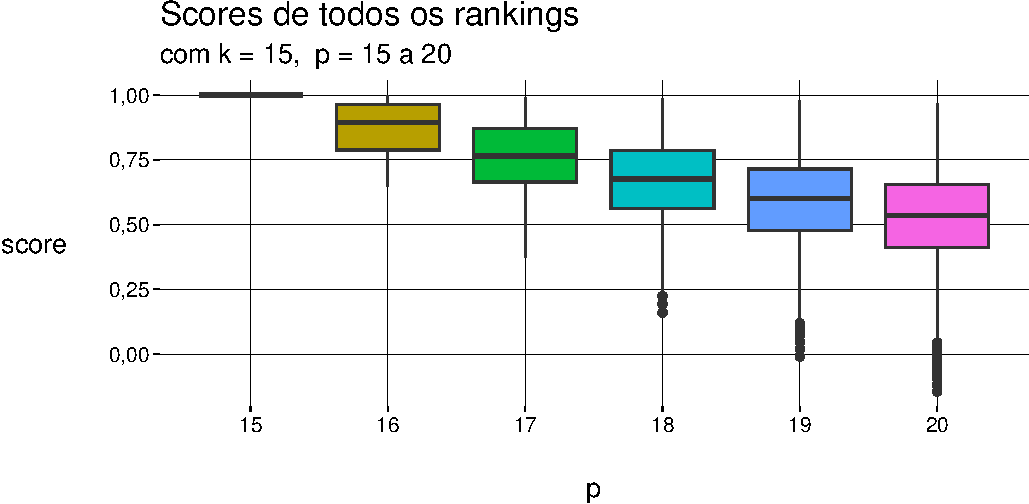
\includegraphics[width=1\textwidth,height=\textheight]{gerar-listas-e-rankings_files/figure-pdf/unnamed-chunk-10-1.pdf}
\end{center}

\begin{Shaded}
\begin{Highlighting}[]
\FunctionTok{plot}\NormalTok{(r, }\AttributeTok{reta =} \ConstantTok{FALSE}\NormalTok{)}
\end{Highlighting}
\end{Shaded}

\begin{center}
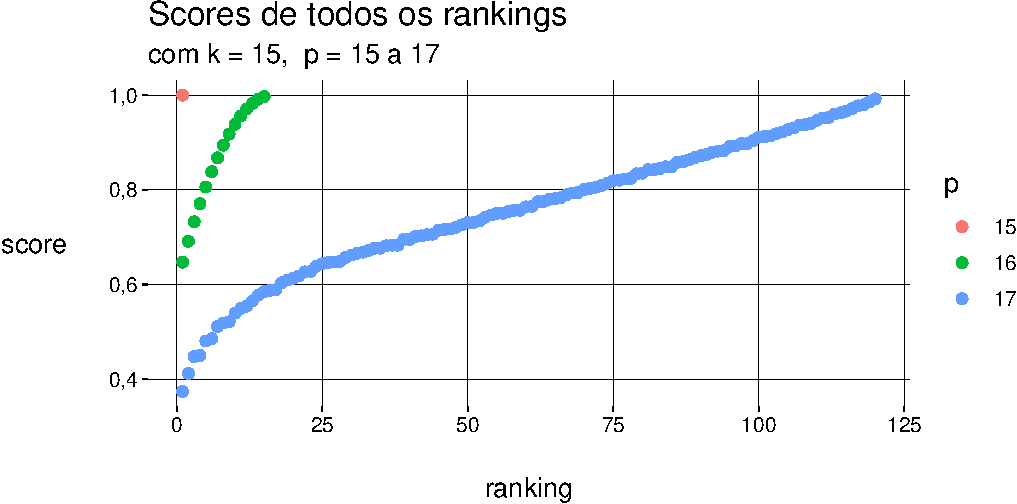
\includegraphics[width=1\textwidth,height=\textheight]{gerar-listas-e-rankings_files/figure-pdf/unnamed-chunk-11-1.pdf}
\end{center}

\begin{Shaded}
\begin{Highlighting}[]
\FunctionTok{plot}\NormalTok{(r, }\AttributeTok{fun =}\NormalTok{ \textbackslash{}(df) \{ }\FunctionTok{cor}\NormalTok{(df}\SpecialCharTok{$}\NormalTok{pos\_lista, df}\SpecialCharTok{$}\NormalTok{pos\_ranking) }\SpecialCharTok{\%\textgreater{}\%} \FunctionTok{round}\NormalTok{(}\DecValTok{2}\NormalTok{) \})}
\end{Highlighting}
\end{Shaded}

\begin{center}
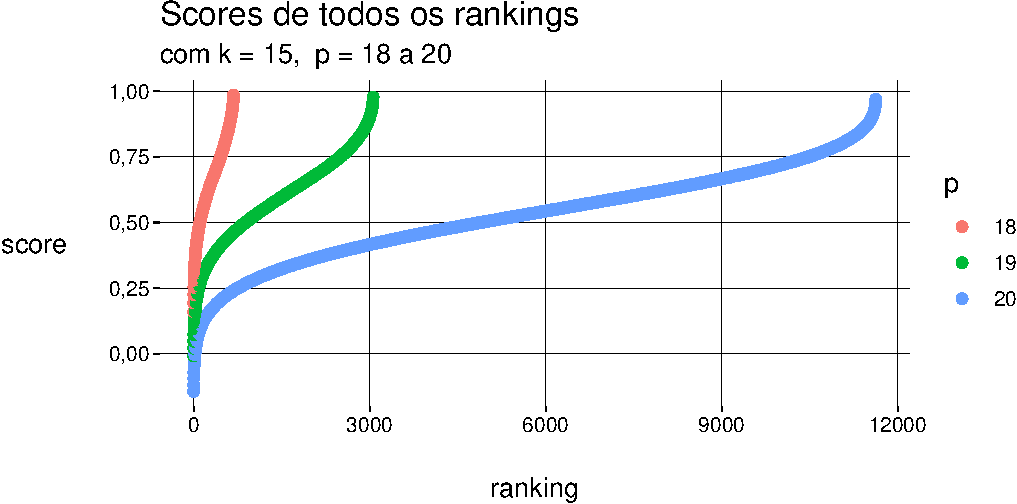
\includegraphics[width=1\textwidth,height=\textheight]{gerar-listas-e-rankings_files/figure-pdf/unnamed-chunk-12-1.pdf}
\end{center}

A função passada em \texttt{fun} deve receber, como único argumento, uma
\emph{tibble} com uma linha para cada elemento, e as colunas

\begin{itemize}
\tightlist
\item
  \texttt{nome}: um vetor de caracteres contendo `\texttt{x}' e
  `\texttt{-}'.
\item
  \texttt{pos\_lista}: um vetor numérico com a posição de cada elemento
  na lista, sendo que elementos do \emph{ranking} que não pertencem à
  lista são adicionados à lista todos empatados no final.
\item
  \texttt{pos\_ranking}: um vetor numérico com a posição de cada
  elemento no \emph{ranking}.
\end{itemize}

\subsection{\texorpdfstring{Criando uma \emph{tibble} com todos os
\emph{rankings}}{Criando uma tibble com todos os rankings}}\label{criando-uma-tibble-com-todos-os-rankings}

Dados valores de $p$ e $k$ (nesta ordem), a função
\texttt{criar\_df\_rankings()} retorna uma \emph{tibble} com todos os
$\binom{p - 1}{k - 1}$ \emph{rankings} possíveis, como objetos (S3) e
como \emph{strings}.

Se for passado apenas o valor de $p$, a função retorna uma \emph{tibble}
com todos os \emph{rankings} possíveis de comprimento $p$ (com $k$
variando de $1$ até $p$). Exercício: quantos são?

Cada \emph{ranking} é representado por um \emph{string}, como descrito
na \hyperref[sec-repr]{seção sobre a representação de \emph{rankings}}.

Todos os \emph{rankings} com $p = 8$ e $k = 5$:

\begin{Shaded}
\begin{Highlighting}[]
\FunctionTok{criar\_df\_rankings}\NormalTok{(}\DecValTok{8}\NormalTok{, }\DecValTok{5}\NormalTok{)}
\end{Highlighting}
\end{Shaded}

\begin{verbatim}
# A tibble: 35 x 2
   ranking ranking_str
   <list>  <chr>      
 1 <rk>    xxxx---x   
 2 <rk>    xxx-x--x   
 3 <rk>    xxx--x-x   
 4 <rk>    xxx---xx   
 5 <rk>    xx-xx--x   
 6 <rk>    xx-x-x-x   
 7 <rk>    xx-x--xx   
 8 <rk>    xx--xx-x   
 9 <rk>    xx--x-xx   
10 <rk>    xx---xxx   
11 <rk>    x-xxx--x   
12 <rk>    x-xx-x-x   
13 <rk>    x-xx--xx   
14 <rk>    x-x-xx-x   
15 <rk>    x-x-x-xx   
16 <rk>    x-x--xxx   
17 <rk>    x--xxx-x   
18 <rk>    x--xx-xx   
19 <rk>    x--x-xxx   
20 <rk>    x---xxxx   
21 <rk>    -xxxx--x   
22 <rk>    -xxx-x-x   
23 <rk>    -xxx--xx   
24 <rk>    -xx-xx-x   
25 <rk>    -xx-x-xx   
26 <rk>    -xx--xxx   
27 <rk>    -x-xxx-x   
28 <rk>    -x-xx-xx   
29 <rk>    -x-x-xxx   
30 <rk>    -x--xxxx   
31 <rk>    --xxxx-x   
32 <rk>    --xxx-xx   
33 <rk>    --xx-xxx   
34 <rk>    --x-xxxx   
35 <rk>    ---xxxxx   
\end{verbatim}

Todos os \emph{rankings} com $p = 5$:

\begin{Shaded}
\begin{Highlighting}[]
\FunctionTok{criar\_df\_rankings}\NormalTok{(}\DecValTok{5}\NormalTok{)}
\end{Highlighting}
\end{Shaded}

\begin{verbatim}
# A tibble: 16 x 2
   ranking ranking_str
   <list>  <chr>      
 1 <rk>    ----x      
 2 <rk>    x---x      
 3 <rk>    -x--x      
 4 <rk>    --x-x      
 5 <rk>    ---xx      
 6 <rk>    xx--x      
 7 <rk>    x-x-x      
 8 <rk>    x--xx      
 9 <rk>    -xx-x      
10 <rk>    -x-xx      
11 <rk>    --xxx      
12 <rk>    xxx-x      
13 <rk>    xx-xx      
14 <rk>    x-xxx      
15 <rk>    -xxxx      
16 <rk>    xxxxx      
\end{verbatim}

Se você quiser a representação em \emph{string} usando unicode, basta
passar o argumento \texttt{unicode\ =\ TRUE}:

\begin{Shaded}
\begin{Highlighting}[]
\FunctionTok{criar\_df\_rankings}\NormalTok{(}\DecValTok{5}\NormalTok{, }\AttributeTok{unicode =} \ConstantTok{TRUE}\NormalTok{)}
\end{Highlighting}
\end{Shaded}

\begin{verbatim}
# A tibble: 16 x 2
   ranking ranking_str
   <list>  <chr>      
 1 <rk>    ••••✔      
 2 <rk>    ✔•••✔      
 3 <rk>    •✔••✔      
 4 <rk>    ••✔•✔      
 5 <rk>    •••✔✔      
 6 <rk>    ✔✔••✔      
 7 <rk>    ✔•✔•✔      
 8 <rk>    ✔••✔✔      
 9 <rk>    •✔✔•✔      
10 <rk>    •✔•✔✔      
11 <rk>    ••✔✔✔      
12 <rk>    ✔✔✔•✔      
13 <rk>    ✔✔•✔✔      
14 <rk>    ✔•✔✔✔      
15 <rk>    •✔✔✔✔      
16 <rk>    ✔✔✔✔✔      
\end{verbatim}

\bookmarksetup{startatroot}

\chapter{\texorpdfstring{O \emph{ranking} concorda com a lista?
Posições}{O ranking concorda com a lista? Posições}}\label{o-ranking-concorda-com-a-lista-posiuxe7uxf5es}

\section{\texorpdfstring{Usando $p$ como medida de
concordância}{Usando  como medida de concordância}}\label{usando-p}

Imagine que a lista de $k$ elementos foi definida por uma autoridade,
usando critérios que não conhecemos.

Em uma tentativa de descobrir esses critérios, construímos um modelo
para avaliar todos os elementos da população (que inclui os $k$
elementos da lista e outros).

Nosso modelo produz um \emph{ranking} de todos os elementos. Para
facilitar, vamos supor que não há empates no \emph{ranking}.

Uma pergunta natural sobre a qualidade do \emph{ranking} produzido é

\begin{quote}
Quantas posições do \emph{ranking} são necessárias para incluir todos os
$k$ elementos da lista?
\end{quote}

A resposta é $p$, a posição, no \emph{ranking}, do elemento da lista com
pior classificação.

Aliás, é por isso que convencionamos, no capítulo anterior, que nossos
\emph{rankings} sempre terminam com um elemento da lista.

Um exemplo:

\begin{itemize}
\item
  A lista contém $k = 5$ elementos.
\item
  O \emph{ranking} $r_1$ é \texttt{xx-x-xx}, com $p = 7$.
\item
  O \emph{ranking} $r_2$ é \texttt{-xxxxx}, com $p = 6$.
\end{itemize}

Segundo a medida proposta aqui, $r_2$ é melhor que $r_1$.

Ou seja, quanto menor o valor de $p$, melhor o \emph{ranking}.

Embora comparar \emph{rankings} através de seus valores de $p$ seja
simples, podemos examinar medidas alternativas, que sejam mais finas que
esta.

Por exemplo, é discutível se os dois rankings \texttt{xx-\/-\/-x} e
\texttt{-\/-\/-xxx} devem ser considerados igualmente bons; no entanto,
ambos têm $p = 6$.

\section{\texorpdfstring{Usando $p$ e as posições dos elementos da
lista}{Usando  e as posições dos elementos da lista}}\label{usando-p-e-as-posiuxe7uxf5es-dos-elementos-da-lista}

\subsection{\texorpdfstring{Contando posições
\texttt{-}}{Contando posições -}}\label{contando-posiuxe7uxf5es--}

Dado um \emph{ranking} $r$ com $k$ e $p$, queremos definir uma função
$s(r)$ com as seguintes características:

\begin{itemize}
\item
  Se $r$ não contiver ``\texttt{-}'', então $s(r) = 1$. Neste caso, $r$
  é um \emph{ranking} perfeito, que coincide com a lista (por exempĺo,
  \texttt{xxxxx}). Em casos assim, $k = p$. Vamos definir $s$ como sendo
  da forma

  \[
  s(r) = \frac k p + \cdots
  \]

  onde as reticências representam termos que ainda vamos definir. Se $r$
  for um \emph{ranking} perfeito, a parcela $k/p$ será $1$, e vamos
  definir os termos restantes para que sejam iguais a zero.
\item
  Os termos restantes devem ter valores maiores quanto melhor for o
  \emph{ranking}. Quanto mais próximos do fim do \emph{ranking}
  estiverem os caracteres ``\texttt{-}'', melhor ele será. Uma
  quantidade natural seria

  \[
  \frac{\operatorname{soma\_}}{\sum_{i = 1, p}i} 
  \quad=\quad 
  \frac{\operatorname{soma\_}}{p(p + 1) / 2}
  \quad=\quad 
  \frac{2\operatorname{soma\_}}{p(p + 1)}
  \]

  onde $\operatorname{soma\_}$ é a soma das posições ocupadas por
  ``\texttt{\_}'' em $r$.

  Como queríamos, quando $r$ for um \emph{ranking} perfeito,
  $\operatorname{soma\_} = 0$, e então $s(r) = 1$.
\item
  Mas também queremos que somente \emph{rankings} perfeitos tenham
  $s(r) = 1$. Para isso, considere que um \emph{ranking} mais próximo do
  perfeito é da forma

  \texttt{x...x-x}

  Ou seja, $k = p - 1$ e $\operatorname{soma\_} = p - 1$.

  Vamos multiplicar a segunda parcela por $\alpha$ de forma que
  $s(r) < 1$ para este \emph{ranking} quase perfeito:

  \[
  s(r) = \frac{p-1}{p} + \frac{2(p-1)}{p(p+1)} \cdot \alpha
  \]

  Então

  \[
  \begin{aligned}
    s(r) < 1 
    &\iff \frac{2(p-1)}{p(p+1)} \cdot \alpha < \frac1p \\
    &\iff 2 \alpha (p - 1) < p + 1 \\
    &\iff \alpha < \frac12 \cdot \frac{p + 1}{p - 1} \\
    &\iff \alpha = \frac1m \cdot \frac{p + 1}{p - 1} & (m > 2)
  \end{aligned}
  \]

  o que dá

  \[
  \begin{aligned}
  s(r) 
  &= \frac{k}{p} + \frac{2\operatorname{soma\_}}{p(p+1)} \cdot \alpha \\
  &= \frac{k}{p} + \frac{2\operatorname{soma\_}}{p(p+1)} \cdot 
    \frac1m \cdot \frac{p + 1}{p - 1} & (m > 2) \\
  &= \frac{k}{p} + \frac{2\operatorname{soma\_}}{p(p-1)} \cdot 
    \frac1m & (m > 2) \\
  &= \frac{k}{p} + \frac{\operatorname{soma\_}}{p(p-1)} \cdot 
    \frac2m & (m > 2)
  \end{aligned}
  \]

  Dependendo do valor de $m > 2$ escolhido, teremos medidas diferentes.

  A função abaixo usa o \emph{default} de $m = 10$, mas valores
  diferentes podem ser passados.
\end{itemize}

\begin{Shaded}
\begin{Highlighting}[]
\NormalTok{s1 }\OtherTok{\textless{}{-}} \ControlFlowTok{function}\NormalTok{(um\_rk, m) \{}
  
\NormalTok{  p }\OtherTok{\textless{}{-}}\NormalTok{ um\_rk}\SpecialCharTok{$}\NormalTok{p}
\NormalTok{  k }\OtherTok{\textless{}{-}}\NormalTok{ um\_rk}\SpecialCharTok{$}\NormalTok{k}
\NormalTok{  soma\_ }\OtherTok{\textless{}{-}} \FunctionTok{sum}\NormalTok{(um\_rk}\SpecialCharTok{$}\NormalTok{no)}

\NormalTok{  (k }\SpecialCharTok{/}\NormalTok{ p) }\SpecialCharTok{+}\NormalTok{ ((}\DecValTok{2} \SpecialCharTok{*}\NormalTok{ soma\_) }\SpecialCharTok{/}\NormalTok{ (m }\SpecialCharTok{*}\NormalTok{ p }\SpecialCharTok{*}\NormalTok{ (p }\SpecialCharTok{{-}} \DecValTok{1}\NormalTok{)))}

\NormalTok{\}}

\NormalTok{s }\OtherTok{\textless{}{-}} \ControlFlowTok{function}\NormalTok{(rk, }\AttributeTok{m =} \DecValTok{10}\NormalTok{) \{}

  \ControlFlowTok{if}\NormalTok{ (}\FunctionTok{is.rk}\NormalTok{(rk)) \{}
    \FunctionTok{s1}\NormalTok{(rk, m)}
\NormalTok{  \} }\ControlFlowTok{else}\NormalTok{ \{}
\NormalTok{    rk }\SpecialCharTok{\%\textgreater{}\%} \FunctionTok{map\_dbl}\NormalTok{(s1, m)}
\NormalTok{  \}}

\NormalTok{\}}
\end{Highlighting}
\end{Shaded}

\begin{verbatim}
[1] 0,84
\end{verbatim}

Para $p = 8$, alguns exemplos:

\begin{Shaded}
\begin{Highlighting}[]
\FunctionTok{s}\NormalTok{(}
  \FunctionTok{list}\NormalTok{(}
    \FunctionTok{rk}\NormalTok{(}\StringTok{\textquotesingle{}xxxxxxxx\textquotesingle{}}\NormalTok{),}
    \FunctionTok{rk}\NormalTok{(}\StringTok{\textquotesingle{}xxxxxx{-}x\textquotesingle{}}\NormalTok{),}
    \FunctionTok{rk}\NormalTok{(}\StringTok{\textquotesingle{}{-}xxxxxxx\textquotesingle{}}\NormalTok{)}
\NormalTok{  )}
\NormalTok{)}
\end{Highlighting}
\end{Shaded}

\begin{verbatim}
[1] 1,0000000 0,9000000 0,8785714
\end{verbatim}

Todos os \emph{rankings} de comprimento $8$, com suas pontuações:

\begin{verbatim}
# A tibble: 128 x 3
    ranking ranking_str     s
    <list>  <chr>       <dbl>
  1 <rk>    xxxxxxxx    1    
  2 <rk>    xxxxxx-x    0.9  
  3 <rk>    xxxxx-xx    0.896
  4 <rk>    xxxx-xxx    0.893
  5 <rk>    xxx-xxxx    0.889
  6 <rk>    xx-xxxxx    0.886
  7 <rk>    x-xxxxxx    0.882
  8 <rk>    -xxxxxxx    0.879
  9 <rk>    xxxxx--x    0.796
 10 <rk>    xxxx-x-x    0.793
 11 <rk>    xxxx--xx    0.789
 12 <rk>    xxx-xx-x    0.789
 13 <rk>    xxx-x-xx    0.786
 14 <rk>    xx-xxx-x    0.786
 15 <rk>    xxx--xxx    0.782
 16 <rk>    xx-xx-xx    0.782
 17 <rk>    x-xxxx-x    0.782
 18 <rk>    xx-x-xxx    0.779
 19 <rk>    x-xxx-xx    0.779
 20 <rk>    -xxxxx-x    0.779
 21 <rk>    xx--xxxx    0.775
 22 <rk>    x-xx-xxx    0.775
 23 <rk>    -xxxx-xx    0.775
 24 <rk>    x-x-xxxx    0.771
 25 <rk>    -xxx-xxx    0.771
 26 <rk>    x--xxxxx    0.768
 27 <rk>    -xx-xxxx    0.768
 28 <rk>    -x-xxxxx    0.764
 29 <rk>    --xxxxxx    0.761
 30 <rk>    xxxx---x    0.689
 31 <rk>    xxx-x--x    0.686
 32 <rk>    xxx--x-x    0.682
 33 <rk>    xx-xx--x    0.682
 34 <rk>    xxx---xx    0.679
 35 <rk>    xx-x-x-x    0.679
 36 <rk>    x-xxx--x    0.679
 37 <rk>    xx-x--xx    0.675
 38 <rk>    xx--xx-x    0.675
 39 <rk>    x-xx-x-x    0.675
 40 <rk>    -xxxx--x    0.675
 41 <rk>    xx--x-xx    0.671
 42 <rk>    x-xx--xx    0.671
 43 <rk>    x-x-xx-x    0.671
 44 <rk>    -xxx-x-x    0.671
 45 <rk>    xx---xxx    0.668
 46 <rk>    x-x-x-xx    0.668
 47 <rk>    x--xxx-x    0.668
 48 <rk>    -xxx--xx    0.668
 49 <rk>    -xx-xx-x    0.668
 50 <rk>    x-x--xxx    0.664
 51 <rk>    x--xx-xx    0.664
 52 <rk>    -xx-x-xx    0.664
 53 <rk>    -x-xxx-x    0.664
 54 <rk>    x--x-xxx    0.661
 55 <rk>    -xx--xxx    0.661
 56 <rk>    -x-xx-xx    0.661
 57 <rk>    --xxxx-x    0.661
 58 <rk>    x---xxxx    0.657
 59 <rk>    -x-x-xxx    0.657
 60 <rk>    --xxx-xx    0.657
 61 <rk>    -x--xxxx    0.654
 62 <rk>    --xx-xxx    0.654
 63 <rk>    --x-xxxx    0.65 
 64 <rk>    ---xxxxx    0.646
 65 <rk>    xxx----x    0.579
 66 <rk>    xx-x---x    0.575
 67 <rk>    xx--x--x    0.571
 68 <rk>    x-xx---x    0.571
 69 <rk>    xx---x-x    0.568
 70 <rk>    x-x-x--x    0.568
 71 <rk>    -xxx---x    0.568
 72 <rk>    xx----xx    0.564
 73 <rk>    x-x--x-x    0.564
 74 <rk>    x--xx--x    0.564
 75 <rk>    -xx-x--x    0.564
 76 <rk>    x-x---xx    0.561
 77 <rk>    x--x-x-x    0.561
 78 <rk>    -xx--x-x    0.561
 79 <rk>    -x-xx--x    0.561
 80 <rk>    x--x--xx    0.557
 81 <rk>    x---xx-x    0.557
 82 <rk>    -xx---xx    0.557
 83 <rk>    -x-x-x-x    0.557
 84 <rk>    --xxx--x    0.557
 85 <rk>    x---x-xx    0.554
 86 <rk>    -x-x--xx    0.554
 87 <rk>    -x--xx-x    0.554
 88 <rk>    --xx-x-x    0.554
 89 <rk>    x----xxx    0.55 
 90 <rk>    -x--x-xx    0.55 
 91 <rk>    --xx--xx    0.55 
 92 <rk>    --x-xx-x    0.55 
 93 <rk>    -x---xxx    0.546
 94 <rk>    --x-x-xx    0.546
 95 <rk>    ---xxx-x    0.546
 96 <rk>    --x--xxx    0.543
 97 <rk>    ---xx-xx    0.543
 98 <rk>    ---x-xxx    0.539
 99 <rk>    ----xxxx    0.536
100 <rk>    xx-----x    0.464
101 <rk>    x-x----x    0.461
102 <rk>    x--x---x    0.457
103 <rk>    -xx----x    0.457
104 <rk>    x---x--x    0.454
105 <rk>    -x-x---x    0.454
106 <rk>    x----x-x    0.45 
107 <rk>    -x--x--x    0.45 
108 <rk>    --xx---x    0.45 
109 <rk>    x-----xx    0.446
110 <rk>    -x---x-x    0.446
111 <rk>    --x-x--x    0.446
112 <rk>    -x----xx    0.443
113 <rk>    --x--x-x    0.443
114 <rk>    ---xx--x    0.443
115 <rk>    --x---xx    0.439
116 <rk>    ---x-x-x    0.439
117 <rk>    ---x--xx    0.436
118 <rk>    ----xx-x    0.436
119 <rk>    ----x-xx    0.432
120 <rk>    -----xxx    0.429
121 <rk>    x------x    0.346
122 <rk>    -x-----x    0.343
123 <rk>    --x----x    0.339
124 <rk>    ---x---x    0.336
125 <rk>    ----x--x    0.332
126 <rk>    -----x-x    0.329
127 <rk>    ------xx    0.325
128 <rk>    -------x    0.225
\end{verbatim}

Perceba que pode haver empates: \texttt{xxxx-\/-xx} e \texttt{xxx-xx-x}
têm o mesmo valor de $s$. É razoável achar que estes dois
\emph{rankings} têm a mesma qualidade.

\subsection{\texorpdfstring{Comparando \emph{rankings} com valores
diferentes de
$p$}{Comparando rankings com valores diferentes de }}\label{comparando-rankings-com-valores-diferentes-de-p}

Como a lista é dada e fixa, só faz sentido, na prática, comparar
\emph{rankings} com o mesmo valor de $k$.

Vamos examinar, para uma lista com $k = 15$, os \emph{rankings}
possíveis com $p$ variando de $15$ a $20$.

São $15.504$ \emph{rankings}. Eis os $100$ melhores:

\begin{verbatim}
# A tibble: 100 x 4
    ranking ranking_str           s     p
    <list>  <chr>             <dbl> <int>
  1 <rk>    xxxxxxxxxxxxxxx   1        15
  2 <rk>    xxxxxxxxxxxxxx-x  0.95     16
  3 <rk>    xxxxxxxxxxxxx-xx  0.949    16
  4 <rk>    xxxxxxxxxxxx-xxx  0.948    16
  5 <rk>    xxxxxxxxxxx-xxxx  0.948    16
  6 <rk>    xxxxxxxxxx-xxxxx  0.947    16
  7 <rk>    xxxxxxxxx-xxxxxx  0.946    16
  8 <rk>    xxxxxxxx-xxxxxxx  0.945    16
  9 <rk>    xxxxxxx-xxxxxxxx  0.944    16
 10 <rk>    xxxxxx-xxxxxxxxx  0.943    16
 11 <rk>    xxxxx-xxxxxxxxxx  0.942    16
 12 <rk>    xxxx-xxxxxxxxxxx  0.942    16
 13 <rk>    xxx-xxxxxxxxxxxx  0.941    16
 14 <rk>    xx-xxxxxxxxxxxxx  0.94     16
 15 <rk>    x-xxxxxxxxxxxxxx  0.939    16
 16 <rk>    -xxxxxxxxxxxxxxx  0.938    16
 17 <rk>    xxxxxxxxxxxxxx--x 0.905    17
 18 <rk>    xxxxxxxxxxxxx-x-x 0.904    17
 19 <rk>    xxxxxxxxxxxxx--xx 0.904    17
 20 <rk>    xxxxxxxxxxxx-xx-x 0.904    17
 21 <rk>    xxxxxxxxxxxx-x-xx 0.903    17
 22 <rk>    xxxxxxxxxxx-xxx-x 0.903    17
 23 <rk>    xxxxxxxxxxxx--xxx 0.902    17
 24 <rk>    xxxxxxxxxxx-xx-xx 0.902    17
 25 <rk>    xxxxxxxxxx-xxxx-x 0.902    17
 26 <rk>    xxxxxxxxxxx-x-xxx 0.901    17
 27 <rk>    xxxxxxxxxx-xxx-xx 0.901    17
 28 <rk>    xxxxxxxxx-xxxxx-x 0.901    17
 29 <rk>    xxxxxxxxxxx--xxxx 0.901    17
 30 <rk>    xxxxxxxxxx-xx-xxx 0.901    17
 31 <rk>    xxxxxxxxx-xxxx-xx 0.901    17
 32 <rk>    xxxxxxxx-xxxxxx-x 0.901    17
 33 <rk>    xxxxxxxxxx-x-xxxx 0.9      17
 34 <rk>    xxxxxxxxx-xxx-xxx 0.9      17
 35 <rk>    xxxxxxxx-xxxxx-xx 0.9      17
 36 <rk>    xxxxxxx-xxxxxxx-x 0.9      17
 37 <rk>    xxxxxxxxxx--xxxxx 0.899    17
 38 <rk>    xxxxxxxxx-xx-xxxx 0.899    17
 39 <rk>    xxxxxxxx-xxxx-xxx 0.899    17
 40 <rk>    xxxxxxx-xxxxxx-xx 0.899    17
 41 <rk>    xxxxxx-xxxxxxxx-x 0.899    17
 42 <rk>    xxxxxxxxx-x-xxxxx 0.899    17
 43 <rk>    xxxxxxxx-xxx-xxxx 0.899    17
 44 <rk>    xxxxxxx-xxxxx-xxx 0.899    17
 45 <rk>    xxxxxx-xxxxxxx-xx 0.899    17
 46 <rk>    xxxxx-xxxxxxxxx-x 0.899    17
 47 <rk>    xxxxxxxxx--xxxxxx 0.898    17
 48 <rk>    xxxxxxxx-xx-xxxxx 0.898    17
 49 <rk>    xxxxxxx-xxxx-xxxx 0.898    17
 50 <rk>    xxxxxx-xxxxxx-xxx 0.898    17
 51 <rk>    xxxxx-xxxxxxxx-xx 0.898    17
 52 <rk>    xxxx-xxxxxxxxxx-x 0.898    17
 53 <rk>    xxxxxxxx-x-xxxxxx 0.897    17
 54 <rk>    xxxxxxx-xxx-xxxxx 0.897    17
 55 <rk>    xxxxxx-xxxxx-xxxx 0.897    17
 56 <rk>    xxxxx-xxxxxxx-xxx 0.897    17
 57 <rk>    xxxx-xxxxxxxxx-xx 0.897    17
 58 <rk>    xxx-xxxxxxxxxxx-x 0.897    17
 59 <rk>    xxxxxxxx--xxxxxxx 0.896    17
 60 <rk>    xxxxxxx-xx-xxxxxx 0.896    17
 61 <rk>    xxxxxx-xxxx-xxxxx 0.896    17
 62 <rk>    xxxxx-xxxxxx-xxxx 0.896    17
 63 <rk>    xxxx-xxxxxxxx-xxx 0.896    17
 64 <rk>    xxx-xxxxxxxxxx-xx 0.896    17
 65 <rk>    xx-xxxxxxxxxxxx-x 0.896    17
 66 <rk>    xxxxxxx-x-xxxxxxx 0.896    17
 67 <rk>    xxxxxx-xxx-xxxxxx 0.896    17
 68 <rk>    xxxxx-xxxxx-xxxxx 0.896    17
 69 <rk>    xxxx-xxxxxxx-xxxx 0.896    17
 70 <rk>    xxx-xxxxxxxxx-xxx 0.896    17
 71 <rk>    xx-xxxxxxxxxxx-xx 0.896    17
 72 <rk>    x-xxxxxxxxxxxxx-x 0.896    17
 73 <rk>    xxxxxxx--xxxxxxxx 0.895    17
 74 <rk>    xxxxxx-xx-xxxxxxx 0.895    17
 75 <rk>    xxxxx-xxxx-xxxxxx 0.895    17
 76 <rk>    xxxx-xxxxxx-xxxxx 0.895    17
 77 <rk>    xxx-xxxxxxxx-xxxx 0.895    17
 78 <rk>    xx-xxxxxxxxxx-xxx 0.895    17
 79 <rk>    x-xxxxxxxxxxxx-xx 0.895    17
 80 <rk>    -xxxxxxxxxxxxxx-x 0.895    17
 81 <rk>    xxxxxx-x-xxxxxxxx 0.894    17
 82 <rk>    xxxxx-xxx-xxxxxxx 0.894    17
 83 <rk>    xxxx-xxxxx-xxxxxx 0.894    17
 84 <rk>    xxx-xxxxxxx-xxxxx 0.894    17
 85 <rk>    xx-xxxxxxxxx-xxxx 0.894    17
 86 <rk>    x-xxxxxxxxxxx-xxx 0.894    17
 87 <rk>    -xxxxxxxxxxxxx-xx 0.894    17
 88 <rk>    xxxxxx--xxxxxxxxx 0.893    17
 89 <rk>    xxxxx-xx-xxxxxxxx 0.893    17
 90 <rk>    xxxx-xxxx-xxxxxxx 0.893    17
 91 <rk>    xxx-xxxxxx-xxxxxx 0.893    17
 92 <rk>    xx-xxxxxxxx-xxxxx 0.893    17
 93 <rk>    x-xxxxxxxxxx-xxxx 0.893    17
 94 <rk>    -xxxxxxxxxxxx-xxx 0.893    17
 95 <rk>    xxxxx-x-xxxxxxxxx 0.893    17
 96 <rk>    xxxx-xxx-xxxxxxxx 0.893    17
 97 <rk>    xxx-xxxxx-xxxxxxx 0.893    17
 98 <rk>    xx-xxxxxxx-xxxxxx 0.893    17
 99 <rk>    x-xxxxxxxxx-xxxxx 0.893    17
100 <rk>    -xxxxxxxxxxx-xxxx 0.893    17
\end{verbatim}

Os gráficos abaixo mostram os \emph{scores} atribuídos para todos os
\emph{rankings} com $k = 15$ e $p$ variando de $15$ a $20$, separados
por valores de $p$:

\begin{center}
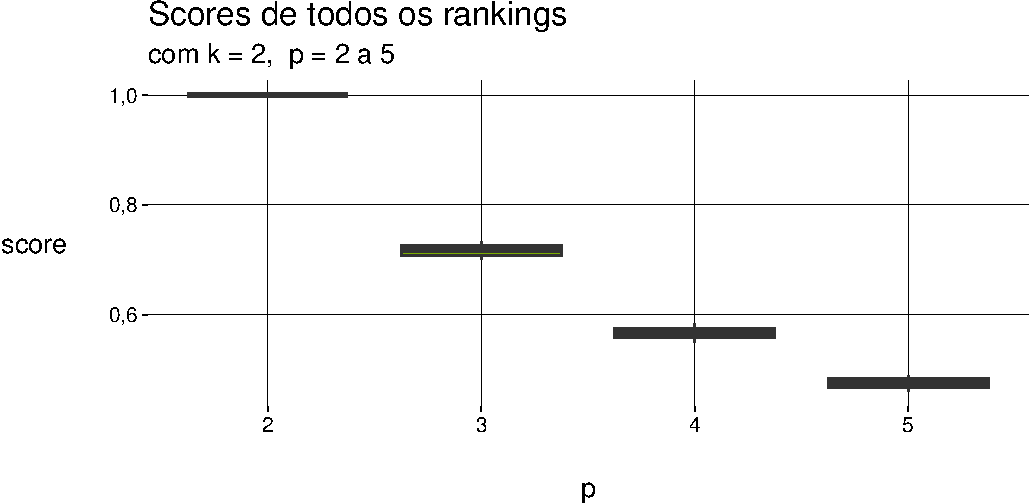
\includegraphics[width=1\textwidth,height=\textheight]{usando-posicoes_files/figure-pdf/unnamed-chunk-7-1.pdf}
\end{center}

\begin{center}
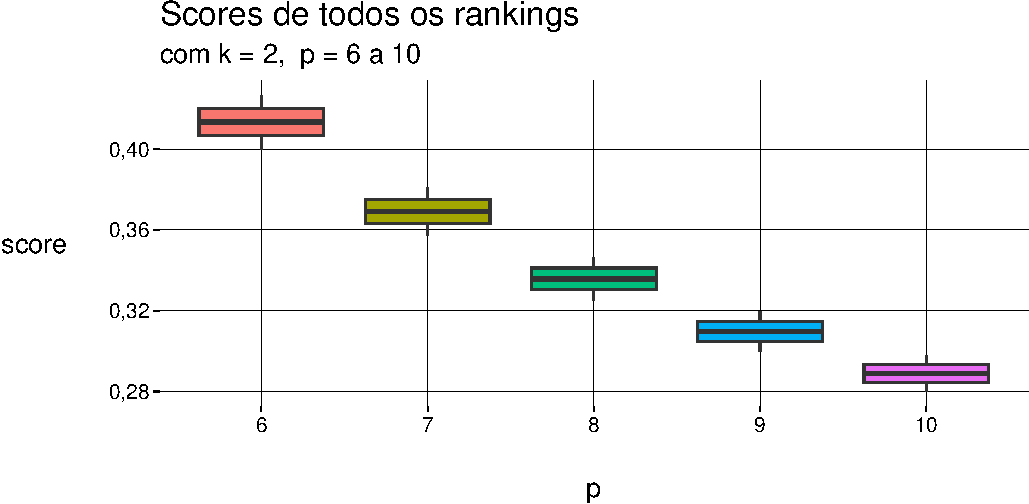
\includegraphics[width=1\textwidth,height=\textheight]{usando-posicoes_files/figure-pdf/unnamed-chunk-8-1.pdf}
\end{center}

\begin{center}
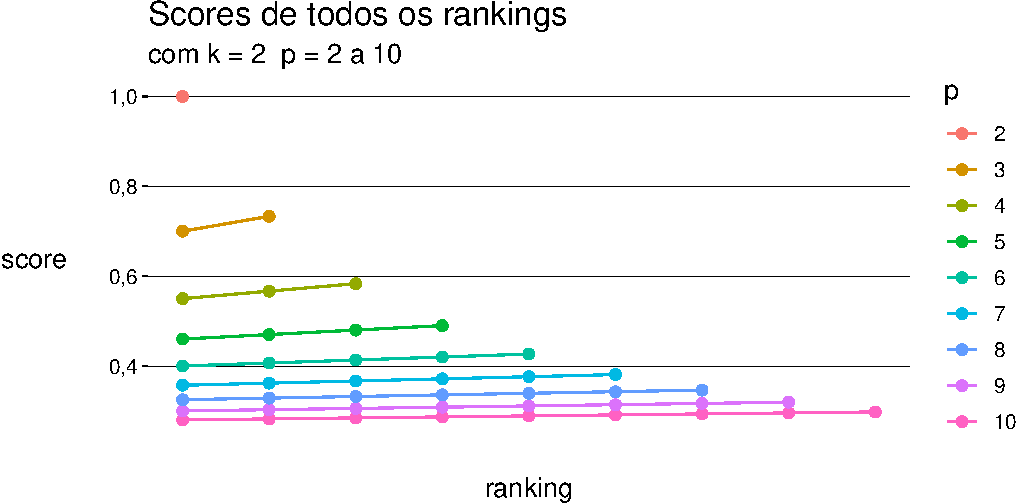
\includegraphics[width=1\textwidth,height=\textheight]{usando-posicoes_files/figure-pdf/unnamed-chunk-9-1.pdf}
\end{center}



\end{document}
